\documentclass{article}

\usepackage{geometry}
 \geometry{
 a4paper,
 left=25mm,
right=25mm,
 top=25mm,
 }

\usepackage{amsmath}
\usepackage{amsthm}
\usepackage{graphicx}
\usepackage{caption}
\usepackage{subcaption}
\graphicspath{ {graphs/} }
\setlength{\parskip}{.3em}

\begin{document}


\section*{Text chunking with Conditional Random Fields under partial feedback simulation}
Conditional Random Fields (CRFs) for sequential prediction have been shown to achieve strong performance in text chunking tasks. Sha and Pereira (2003) showed that Conditional Random Fields achieved performance as good as any other reported models in the Noun Phrase chunking CoNLL-2000 data task. Here, we replicated the results of Sha and Pereia's CRF implementation, and then modified the model to learn under partial-feedback simulation. 

\subsection*{Conditional Random Fields formulation}
We assume the classical chain Conditional Random Field described in Klinger et al. (2007), with the general theory of CRF proposed by in Lafferty et al. (2001), Taskar et al. (2002). CRFs describe a discriminative structured model $p(\vec{y}|\vec{x})$, where in our situation $x_{i}$ in $\vec{x}$ describes the words and POS tags of a sentence $\vec{x}$, and $y_{i}$ in $\vec{y}$ describes the chunk tag label of each word. Each chunk tag label can take on three possibilities: ${B, I, O}$, denoting beginning, inside, or outside of a Noun Phrase, respectively. These chunk tags are non-recursive. 

A linear-chain CRF can been seen as a hybrid of Hidden Markov Models (HMMs) and Maximum Entropy Log-Linear models.  The typical setup for HMMs, such as $p(\vec{y},\vec{x})=\prod_{t}^{T}p(y_{t}\mid y_{t-1})p(x_{t}\mid y_{t})$ can be rewritten in a conditional form using binary features. The features tell the relationship between the $y_{t}$ and $y_{t+1}$ labels and the relationship between the input $x_{t}$ and label $y_{t}$: $f_{pairwise}(y_{t},y_{t-1},i,j)=1_{y_{t}=i}1_{y_{t-1}=j}$,
$f_{unary}(y_{t}x_{t},j,k)=1_{y_{t}=j}1_{x_{t}=k}$. Throwing in a $log$ and $exp$, we get a Log-Linear form: 
\begin{equation}
\label{CRF1}
p(\vec{y}|\vec{x})=\frac{p(\vec{y},\vec{x})}{\sum_{\vec{y'}}p(\vec{y'},\vec{x})}=\frac{\prod_{t=1}^{T}exp(\sum_{j}\lambda_{j}f_{j}(y_{t},y_{t-1},x_{t}))}{Z(\vec{x})}
\end{equation}
where the indicies $i, j, k$ described in the features are reordered into one general index $j$ listing all pairwise and unary features. This derivation from HMMs to CRFs can be seen in more detail through Sutton's (2006) introduction of CRFs. 

This first form of CRFs is often rewritten slightly differently for both computational purposes and to emphasize the flexibility of feature choice. Let $M_{t}(\vec{x})$ be a set of $T-1$ matrices, each size of $|Y| \times|Y|$ where $Y$ is the set of labels: $M_{t}(y',y|\vec{x})=exp(\sum_{j}\lambda_{j}f_{j}(y',y,\vec{x},i))$. Then \ref{CRF1} can be rewritten as:
\begin{equation}
\label{CRF2}
p(\vec{y}|\vec{x})=\frac{\prod_{t=1}^{T-1}M_{t}(y_{t-1},y_{t}|\vec{x})}{Z(\vec{x})}
\end{equation}
In this form, $M_{t-1}(y_{t-1}, t_{t}|\vec{x})$ gives the $potentials$ of going from label $y_{t-1}$ to $y_{t}$ ($y_{i}$ is indexed from $0$ to $|Y|-1$). This form emphasizes that CRFs differ greatly from HMMs in the sense that 
\begin{enumerate}
\item it is an undirected graphical model as opposed to an directed graphical model so the potentials do not necessarily have a probabilistic interpretation and 
\item features can have a much flexible definition, similar to the setup of Maximum Entropy Log-Linear models.
\end{enumerate}

The details of inference (Forwards-Backwards algorithm) and decoding (Viterbi) for CRFs are similar to the story of HMMs. Following the theory of Maximum Entropy models, the expected value of features under model distribution should equal the expected value of features under empirical distribution. Computing the gradient of the log-likelihood indeed results in $\nabla\lambda_{k}=\tilde{E}(f_{k})-E(f_{k})=0$. 


\subsection*{Implementation on text chunking}
Sha and Pereira's implementation of CRFs for text chunking had a few important modifications to general linear-chain CRFs. First, the model incorporated second-order Markov dependency (bigram dependency), so for label at position $i$, $y_{i}=c_{i-1}c_{i}$, where $c_{i}$ is the chunk tag of word $i$. This increases our possible labels, $|Y|$, to $9$ instead of $3$. Second, impossible labels and label sequences such as $OI$ and $\textunderscore O \rightarrow I\textunderscore$ are omitted by giving them a feature weight of $-\infty$. We used the CoNLL-2000 dataset, splitting into $train$ of 7936 sentences and $dev$ of 1000 sentences. A seperate $test$ dataset was given with 2012 sentences.

The complete list of features used are described in the Sha and Pereira's paper. We made a quick estimate of total number of features that can be generated by the train dataset, and the number was around the range of 5 billion. An actual count of generated features in the train dataset upon running the model was just under 2 million. We stored our features and weights in a sparse array with a hash size of 2 million entries.

In our implementation to recreate the work of Sha and Pereira's CRF model, we followed everything as above with a few minor changes. First, in the original proposal of CRFs, two additional labels, $\{S, F\}\in Y$ denoting start and finish, are included in the labels to model the first and last labels' probabilities.  We dismissed them in our implementation as the inclusion of them made no significant numerical difference in the task performance. Second, two pairwise feature sets described in Sha and Pereira's list of features, $y_{i}=y$ and $c(y_{i})=c$ were also left out due to difficulties in implementation. We felt these these omissions are reasonable as without them, our reimplementation of the chunking experiment under full information was comparable to that of Sha and Pereira's. 

Our evaluation metric is the F1 score, the geometric mean of precision and recall for noun phrases.

\subsection*{Implementation for partial feedback simulation}

To learn from partial feedback, we need to sample from the model distribution. We propose the following method to sample a structure from the model distribution: given $y_{i} \in \vec{y}$, $$y_{i+1}\sim Multinominal\left(M_{i+1}(y_{i,}1)\cdot\beta_{i+1}(1),\: M_{i+1}(y_{i,}2)\cdot\beta_{i+1}(2),\:...\:,M_{i+1}(y_{i,}n)\cdot\beta_{i+1}(n)\right)$$,
 where $n:=|Y|$ and $\beta$ comes from the Forwards-Backwards algorithm. For one sample of length $T$, we sampled $T$ times. 

\begin{proof}
The above sampling method can be rewritten as: $\tilde{p}_i(y_i|y_{i-1}) = \frac{M_i[y_{i-1}, y_i]\beta[y_i]}{\sum_y M_i[y_{i-1}, y]\beta[y]}$. Then,
\begin{align*}
  \tilde p(\tilde y) 
 &=\tilde p(y_0,\dots,y_{T})\\
 &= \prod_{i=1}^{T} \tilde p_i(y_i|y_{i-1})&& \text{(by independence)}\\
 &= \prod_{i=1}^{T} \frac{M_i[y_{i-1}, y_i]\beta[y_i]}{\sum_y M_i[y_{i-1}, y]\beta_i[y]}\\
 &= \prod_{i=1}^{T} \frac{e^{\lambda f(x,y_{i-1},y_i)}\beta[y_i]}{\sum_y M_i[y_{i-1}, y]\beta_i[y]}\\
 &= e^{\lambda f(x,\tilde y)} \cdot \prod_{i=1}^{T} \frac{\beta_i[y_i]}{\sum_y M_i[y_{i-1}, y]\beta_i[y]}\\
 &= e^{\lambda f(x,\tilde y)} \cdot \prod_{i=1}^{T} \frac{\beta_i[y_i]}{\beta_{i-1}[y_{i-1}]}&& \text{(by definition of $\beta$)}\\
 &= e^{\lambda f(x,\tilde y)} \frac{1}{\beta_{0}[y_{0}]}\\
 &= e^{\lambda f(x,\tilde y)} \frac{1}{Z(x)}&& \text{(by original formulation of CRFs in Laffety et al.)}\\
 &= p_{\text{model}}(\tilde y|x;w)
 \end{align*}
\end{proof}

\subsection*{Experimental results}
For our full information experiments as a baseline to compare to partial-feedback simulations, we attained a F1 score of 92.8 on $test$, which is comparable with Sha and Pereira's  F1 score of 94.38. 

For the Bayes loss function, we obtained a F1 score of $91.29$ on $test$, which is comparable with many other full information models that performed the CoNLL-2000 data task. For Pairwise Bayes, we obtained a F1 score of 90.54 on $test$. 

For the cross entropy loss function, we had more difficulties maximizing the gain function. Although cross entropy is a convex loss function, the difficulty of convergence arises from high variance in the gradient decent. The term $\frac{g(\tilde{y_{t}})}{p_{w}(\tilde{y_{t}}|x_{t})}$ creates extremely high variance as the numerator, $g(\tilde{y_{t}})$, clustered around $10^{-3}$ to $10^{-1}$ while the denominator, $p_{w}(\tilde{y_{t}}|x_{t})$, clustered around $10^{-40}$ to $10^{-10}$. Therefore, $Var(\frac{g(\tilde{y_{t}})}{p_{w}(\tilde{y_{t}}|x_{t})})$ was gigantic. Dividing $p_{w}(\tilde{y_{t}}|x_{t})$ by a normalization term that reflected the number of possible structured labels $nodes^{\frac{|Y|}{c}}$, where $c=.5$, reduced this variance. The update term became more stable with ranges $10^{-5}$ to $10^{-1}$, and we were able to achieve a sub-par F1 score of 65.06 on $test$. See Figure 1 for comparison. 

\begin{figure}[h]
\centering
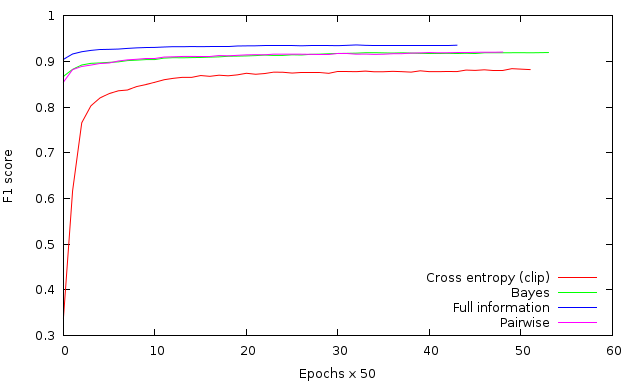
\includegraphics[scale=.35]{output}
\caption{Learning curves for full information, bayes, pairwise, and cross entropy on $dev$ set, all with learning rate of $\gamma=.001$ and regularization rate of $\lambda=.0000$1.}
\end{figure}

We tried several techniques to improve the performance of the cross entropy loss function. 

\begin{enumerate}
\item The classical momentum (CM) method (Polyak, 1964) is a technique for accelerating gradient decent that creates velocity accumulation of gradients. The method did not improve the situation.
\item The ADADELTA method (Zeiler, 2012) tunes per-dimension learning rate for gradient descent. We thought that ADADELTA may help as it has been shown effective in sparse situations, but the method did not improve the situation. 
\item Simulated full information out-of-domain learning on a small dataset (25 sentences and 200 sentences, carved out of $train$) before transferring to cross entropy learning performed surprisingly poorly. Using full information models with F1 scores of 75$\%$ and 85$\%$  from the 25 sentences and 200 sentences dataset respectively,  the model immediately returned to its previous cross entropy state in terms of F1 score once the method of learning transferred to the cross entropy update. This means that loss/gain functions of Bayes and cross entropy are significantly different.  
\item Clipping low probability values of $p_{w}(\tilde{y_{t}}|x_{t})$ below a threshold $c$ to $c$ yieled promising benefits.  As we increased the threshold of clipping, the percentages of sentences that are clipped increased so the update became more similar to Bayes as $p_{w}(\tilde{y_{t}}|x_{t})$  approached a constant.  We cannot say that this modified clipping stochastic gradient update will converge to the optimum of the cross entropy loss function, as $\nabla J(w_{t}) \cdot  E (s_{t})$ will not necessary be greater than or equal to $0$, where $$E(s_{t})=\sum_{y}\Delta \tilde{y}[\phi - E(\phi)]1[p \geq c] + \sum_{y}\frac{p}{c}\Delta \tilde{y}[\phi - E(\phi)]1[p<c]$$.

However, if the percentage of sentences that are clipped decreases while the model improves, the update becomes similar to the cross entropy update. We tested several clipping thresholds to see whether the percentage of number of sentences clipped decreased as the model improved. It is intuitive to expect that the percentage of sentences that are clipped to decrease but we cannot say how much it will, if at all, decrease. 

We found that with parameters $\gamma=.0001$, $c=.05$, we got our best clipped cross entropy model of 87.72 on $test$, but 64.17$\%$ of sentences per epoch at decode were clipped, so the update is "more Bayes than cross entropy". With a desire to minimize the clip percentage at decode, we were also able to achieve a promising F1 score of 80.31 on $test$ with clip percentage of $.6175\%$, which is "mostly cross entropy and a little bit of Bayes".   The effects of learning rate and clipping thresholds are detailed in Table 1. The relationships of F1 score, clip percentage, and clip thresholds are detailed in Figure 2.




\end{enumerate}

\begin{table}[h]
\centering
\begin{tabular}{l|l|l|l|l}
Learning rate & $p_{w}(\tilde{y_{t}}|x_{t})$ clip threshold& Clip percentage at decode & F1 on $dev$ & F1 on $test$\\
\hline
.01 & .05 & .6175$\%$ & 80.57 & 80.32 \\
\hline
.01 & .005 & .0003780$\%$ & 60.09 & 59.74 \\
\hline
.001 & .05 & 23.51$\%$ & 79.23 & 78.39 \\
\hline
.001 & .005 & .004102$\%$ & 66.44 & 66.01\\
\hline
.001 & .0005 & 0$\%$ & 49.16 & 48.35\\
\hline
.0001 & .05 & 64.17$\%$ & 88.12 & 87.72\\
\hline
.0001 & .005 & .5419$\%$ & 65.35 & 64.98\\
\hline
.0001 & .0005 & 0$\%$ & 48.74 & 47.60\\
\hline
.00001 & .05 & 69.91$\%$ & 87.53 & 87.11 \\
\hline
.00001 & .005 & 65.58$\%$ & 80.06 &79.36 \\
\hline
.00001 & .0005 & 37.50$\%$ & 61.32 & 60.85  \\
\end{tabular}
\caption{Effects of clip threshold on clip percentage and F1 score, with regularization rate of $\lambda=.00001$.}
\end{table}

\begin{figure*}[t!]
    \centering
    \begin{subfigure}[t]{0.5\textwidth}
        \centering
       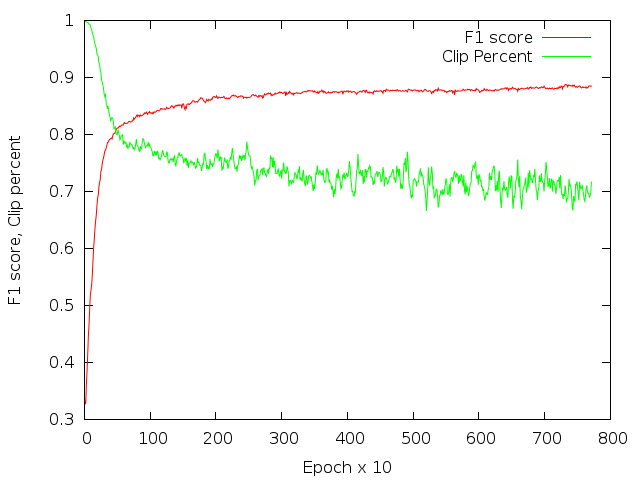
\includegraphics[scale=.2]{output05}
        \caption{$c=.05$}
    \end{subfigure}%
    ~ 
     \begin{subfigure}[t]{0.5\textwidth}
        \centering
       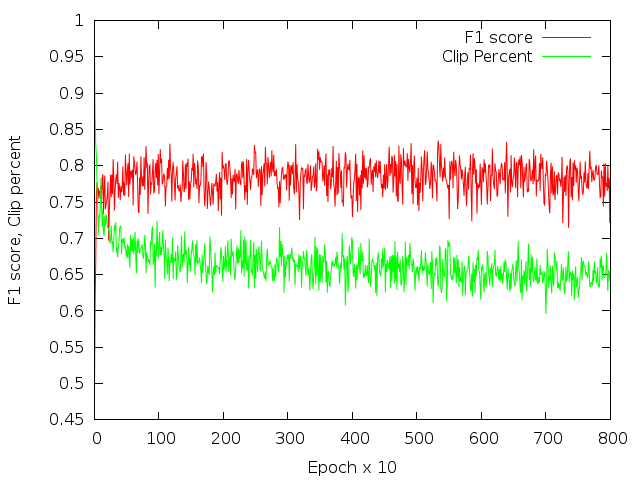
\includegraphics[scale=.2]{output005}
        \caption{$c=.005$}
    \end{subfigure}%

  \begin{subfigure}[t]{0.5\textwidth}
        \centering
       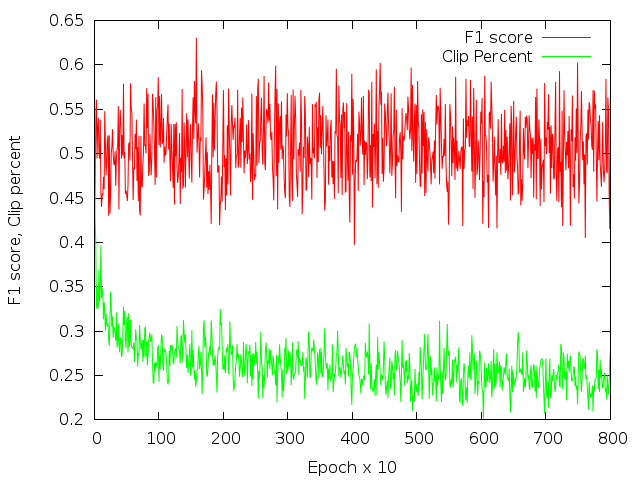
\includegraphics[scale=.2]{output0005}
        \caption{$c=.0005$}
    \end{subfigure}%
~
  \begin{subfigure}[t]{0.5\textwidth}
        \centering
       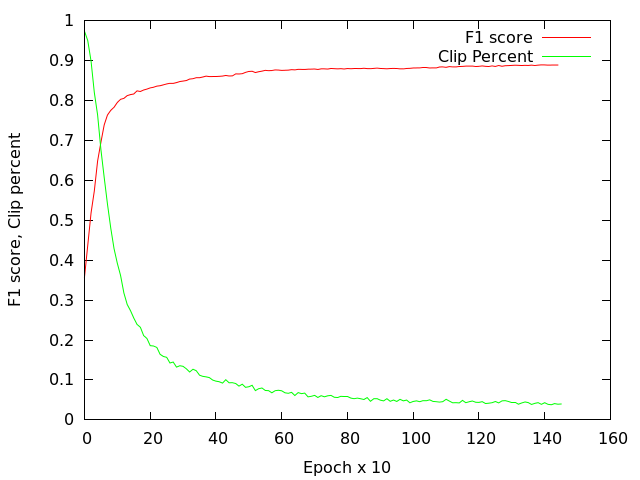
\includegraphics[scale=.2]{bayes}
        \caption{Bayes, $c=.005$}
    \end{subfigure}%
    \caption{Cross entropy with clipping thresholds $c=.05, .005, .0005$ with learning rate and regularization rate held at $\gamma=\lambda=.00001$. We also included the Bayes update in which we examined $p_{w}(\tilde{y_{t}}|x_{t})$ without modifying the update. The clip percent measures the number of sentences in an epoch that were clipped as a result of sampling probability below $c$. With a higher clipping threshold, the model update becomes more like the Bayes update, with less variance and better F1 score performance on $dev$.}
\end{figure*}





\end{document}